%%%%%%%%%%%%%%%%%%%%%%%%%%%%%%%%%
\chapter{クイーン支配問題の制約モデル}\label{chap:constraint}
%%%%%%%%%%%%%%%%%%%%%%%%%%%%%%%%%
本章では,SATソルバーを用いた既存研究~\cite{yamamoto21}で
提案された制約モデルである,基本モデル,改良モデル,部分和モデル
についての説明を行う.
各制約モデルにおいて,
入力はクイーングラフ$Q_{n}$と正の整数$k$である.

\section{基本モデル}
\begin{description}
 \item[(変数$q_{ij}$)] $q_{ij} \in \{0,1\}$ \par
1のとき,マス$(i,j)$にクイーンが配置されることを意味する.
 \item[(制約1)] $\sum\limits_{i,j=1}^{n} q_{ij} = k$ \par
クイーングラフ上のクイーンの総数が$k$であることを意味する.
 \item[(制約2)] $(\bigvee\limits_{(i',j')\in A_{ij}} q_{i'j'}) >0 \qquad (1 \leq i,j \leq n)$ \par
マス$(i,j)$に1つ以上のクイーンが移動できることを意味する.
ここで,$A_{ij}$はマス$(i,j)$と$Q_n$上で隣接している頂点の集合を表す.
\end{description}

このモデルを$n=3,k=2$で実行すると,コード~\ref{code:3-2_model0}のように変数と節が生成される.なお,コード~\ref{code:3-2_model0}において,\code{(int  q_i_j  0  1)}は\code{q_i_j}が0または1の値を取る変数であること,\code{(= (+ q_1_1 ... q_3_3) 2)}は\code{(q_1_1 + ... + q_3_3 = 2)}であること,\code{(> (+ q_1_1 ... q_3_3) 0)}は\code{((q_1_1 + ... + q_3_3) > 0)}であることを表す.

生成された節に着目すると,(制約2)で生成される節において,例えば16-18行目の\code{(+ q_1_1 q_1_2 q_1_3 ...)}のように同じ部分式が複数の節で出現していることがわかる.
\lstinputlisting[float=ht,caption={%
基本モデルの実行例($n=3,k=2$)},%
captionpos=b,frame=single,label=code:3-2_model0,%
numbers=none,%
breaklines=true,%
columns=fullflexible,keepspaces=true,%
basicstyle=\ttfamily\scriptsize]{code/qdp_3-2_model0.log}

%\newpage
\section{改良制約モデル}
本モデルでは,基本制約モデルにおいて複数回出現する部分式をまとめるための補助ブール変数と制約を追加する.

各行に対して以下の補助ブール変数と制約を追加する.
\begin{description}
 \item[(変数$r_i$)] $r_{i} \in \{0,1\} \qquad (1 \leq i \leq n)$\par
  1のとき,行$i$にクイーンが1つ以上存在することを意味する.
 \item[(制約3)] $r_{i}>0 \rightarrow \bigvee\limits_{(i',j')\in R_{i}} q_{i'j'}=1 \qquad (1 \leq i \leq n)$ \par
  $r_{i}$が1のとき,行$i$上にクイーンが1つ以上配置されていることを意味する.
  ここで,$R_i$は行$i$上に存在する頂点の集合を表す.
\end{description}
%
各列,各右上がり対角線,各右下がり対角線についても同様に,
補助ブール変数$c_{j}$,$u_{a}$,$d_{b}$を追加し,
(制約4),(制約5),(制約6)を追加する.
%
\begin{description}
 \item[(制約4)] $c_{j}>0 \rightarrow \bigvee\limits_{(i',j')\in C_{j}} q_{i'j'}=1 \qquad (1 \leq j \leq n)$ 
 \item[(制約5)] $u_{a}>0 \rightarrow \bigvee\limits_{(i',j')\in U_{a}} q_{i'j'}=1 \qquad (1 \leq a \leq 2n-1)$ 
 \item[(制約6)] $d_{b}>0 \rightarrow \bigvee\limits_{(i',j')\in D_{b}} q_{i'j'}=1 \qquad (1 \leq b \leq 2n-1)$ \par
  ここで,$C_j$,$U_{a}$,$D_{b}$はそれぞれ列$j$,右上がり対角線$a$,
  右下がり対角線$b$上に存在する頂点の集合を表す.
\end{description}

さらに,基本制約モデルの(制約2)を削除し,以下の(制約7)に置き換える.
\begin{description}
 \item[(制約7)] $(r_i > 0) \vee (c_j >0) \vee (u_{a}>0) \vee (d_{b}>0) \qquad (1 \leq i,j \leq n)$
\end{description}

このモデルを$n=3,k=2$で実行すると,コード~\ref{code:3-2_model1}のように変数と節が生成される.なお,コード~\ref{code:3-2_model1}において,\code{(imp (> r_1 0) }\code{(> (+ q_1_1 q_1_2 q_1_3) 0))}は\code{((r_1 > 0)} $\rightarrow$ \code{(q_1_1 + q_1_2 + q_1_3 > 0))}であること,\code{(or (> r_1 0) } \code{(> c_1 0) } \code{(> u_1 0)} \code{(> d_3 0))}は\code{(r_1 > 0} $\vee$ \code{c_1 > 0} $\vee$ \code{u_1 > 0} $\vee$ \code{d_1 > 0)}を表す.
\lstinputlisting[float=ht,caption={%
改良モデルの実行例($n=3,k=2$)},%
captionpos=b,frame=single,label=code:3-2_model1,%
numbers=none,%
breaklines=true,%
columns=fullflexible,keepspaces=true,%
basicstyle=\ttfamily\scriptsize]{code/qdp_3-2_model1.log}


%\newpage
\section{部分和モデル}
本モデルでは,クイーンの個数を表す補助整数変数を追加し,
行方向,列方向,対角線方向のクイーンの総数に関する制約を追加する.
\begin{description}
 \item[(変数$r_i$)] $r_{i} \in \{0,...,k\}$ 
 \item[(制約8)] $r_{i} = \sum\limits _{(i',j') \in R_{i}} q_{i'j'} \qquad (1 \leq i \leq n)$ \par
$r_i = s$のとき,行$i$にクイーンが$s$個存在することを意味する.
\end{description}
%
各列,各右上がり対角線,各右下がり対角線に対しても同様に
補助整数変数$c_j$,$u_{a}$,$d_{b}$と(制約9),(制約10),(制約11)を追加する.
%
\begin{description}
 \item[(制約9)] $c_{j} = \sum\limits _{(i',j') \in C_{j}} q_{i'j'} \qquad (1 \leq i \leq n)$
 \item[(制約10)] $u_{a} = \sum\limits _{(i',j') \in U_{a}} q_{i'j'}\qquad (1 \leq a \leq 2n-1)$
 \item[(制約11)] $d_{b} = \sum\limits _{(i',j') \in D_{b}} q_{i'j'} \qquad(1 \leq b \leq 2n-1)$
\end{description}
さらに,クイーンの総数に関する制約である(制約12)を追加する.
\begin{description}
 \item[(制約12)] $\sum\limits_{i=1}^{n} r_{i} = \sum\limits_{j=1}^{n} c_{j} =\sum\limits_{a=1}^{2n-1} u_{a} =\sum\limits_{b=1}^{2n-1} d_{b} = k$ \par
各行,各列,各対角線ごとにクイーンの個数を足し合わせるとクイーンの総数$k$に等しいことを意味する.\par

部分和モデルにより起こる制約伝播を図~\ref{fig:constraint}に示す.説明のため,上から行1,行2, \dots , 行5とする.まず,図~\ref{fig:constraint}の赤丸のマスを被覆するために行1にクイーンが置かれなければならない.同様に,図~\ref{fig:constraint}の青丸のマスを被覆するために行2にクイーンが置かれなければならない.そして,図~\ref{fig:constraint}のオレンジ色のマスを被覆するために行5にクイーンが置かれなければならない.以上から,$r_1 \geq 1$かつ$r_2 \geq 1$かつ$r_5 \geq 1$である(図~\ref{fig:constraint}の左の状態).さらに,(制約12)より,$\sum\limits _{i=1}^{5} r_i = 3$であることから,$r_1 = 1,r_2=1,r_3=0,r_4=0,r_5=1$であることがわかり,図~\ref{fig:constraint}の右の図のように制約伝播が起こる.

\begin{figure}[htb]
  \centering
  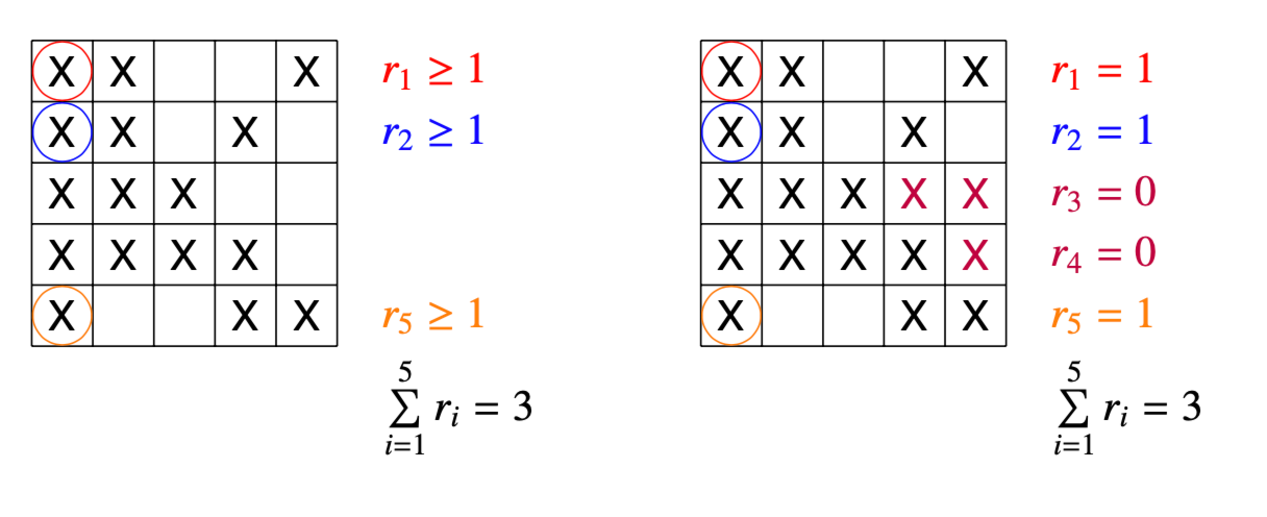
\includegraphics[width=1 \linewidth]{fig/fig-constraint.pdf}
  \caption{部分和モデルにおける制約伝播の例}
  \label{fig:constraint}
\end{figure}

このモデルを$n=3,k=2$で実行すると,コード~\ref{code:3-2_model2}のように変数と節が生成される.なお,\code{(int r_1 0 2)}は\code{r_1}が0,1,2のいずれかの値をとる整数変数であることを表す.
\lstinputlisting[float=ht,caption={%
部分和モデルの実行例($n=3,k=2$)},%
captionpos=b,frame=single,label=code:3-2_model2,%
numbers=none,%
breaklines=true,%
columns=fullflexible,keepspaces=true,%
basicstyle=\ttfamily\scriptsize]{code/qdp_3-2_model2.log}

\end{description}